% Inbuilt themes in beamer
\documentclass[aspectratio=169]{beamer}

% Theme choice:
\usetheme{CambridgeUS}
\usecolortheme{orchid}
\setbeamertemplate{navigation symbols}{} % Remove navigation buttons

% Auto make section slides
% from https://statisticaloddsandends.wordpress.com/2019/02/18/beamer-inserting-section-slides-before-each-section/
\AtBeginSection[]
{
    \begin{frame}
        \frametitle{Table of Contents}
        \tableofcontents[currentsection]
    \end{frame}
}

%% Get better (serif) math font
\usefonttheme{professionalfonts}

\usepackage{xcolor}

\usepackage{tikz}
\usetikzlibrary{tikzmark}
\usetikzlibrary{shapes, arrows, calc, math, positioning, shapes.misc}
\tikzstyle{block} = [rectangle, draw, text width = 40mm, text centered, rounded corners, minimum height = 1.5\baselineskip]
\tikzstyle{line} = [draw, -latex']
\tikzset{cross/.style={cross out, draw=black, minimum size=2*(#1-\pgflinewidth), inner sep=0pt, outer sep=0pt},
%default radius will be 1pt. 
cross/.default={1pt}}

\tikzset{
    cg/.pic = {
    \fill[fill=black] (0,0) -- (#1,0) arc (0:90:#1) -- cycle;
    \fill[fill=white] (0,0) -- (0,#1) arc (90:180:#1) -- cycle;
    \fill[fill=black] (0,0) -- (-#1,0) arc (180:270:#1) -- cycle;
    \fill[fill=white] (0,0) -- (0,-#1) arc (270:360:#1) -- cycle;
    \draw (0,0) circle (#1);
    }
}

% Title page details:
\title{Racecar 101}
\author{James Wright}
% \date{\today}
% \logo{\large \LaTeX{}}

\begin{document}

% Title page frame
\begin{frame}
    \titlepage
\end{frame}

% Remove logo from the next slides
\logo{}

% Outline frame
\begin{frame}{Outline}
    \tableofcontents
\end{frame}

\begin{frame}
    \begin{alertblock}{Note}
        This first part is a very simplified breakdown
        \begin{itemize}
            \item It's not the most accurate
            \item It's not to insult anyone's intelligence
        \end{itemize}
        It's simply to not distract from the things that can be easily
        forgotten or muddied.
    \end{alertblock}

    Also, I like audience participation. Ask questions. I'll be asking y'all questions.
\end{frame}

\section{What makes a car fast?}

\begin{frame}{What makes a car go fast?}

    \onslide<+-> {
        \begin{equation*}
            \mathrm{Time} = \frac{\mathrm{Distance}}{\mathrm{Velocity}}
        \end{equation*}
    }

    \begin{itemize}
        \onslide<+->{\item To lower time, we need to increase velocity\footnote{Assuming distance is constant}}
        \item<+-> All motorsports have velocity changes during a race
            \begin{itemize}
                \item Excluding top-speed records of course
            \end{itemize}
        \item<+-> Change in velocity is... \onslide<+->{\textbf{Acceleration}}
        \item<+-> To maximize velocity, you must maximize acceleration
            \begin{itemize}
                \item ie. Whatever changes in velocity you make, do them as quickly as possible
            \end{itemize}
        \begin{block}{}<+->
            To make a car \textbf{faster}, you must make the car \textbf{accelerate more}
        \end{block}
    \end{itemize}

\end{frame}

\begin{frame}{What famous equation involves acceleration?}
    \onslide<2->{
        \center Newton's 2nd law!
        \begin{equation*}
            F=ma
        \end{equation*}
    }

    \onslide<3->{
        We care about acceleration, so rearange:
        \begin{equation*}
            a = \frac{F}{m}
        \end{equation*}
    }
\end{frame}

\begin{frame}{How do we maximize acceleration?}
    \begin{equation*}
        a = \frac{F}{m}
    \end{equation*}

    \begin{block}{Decrease Mass}<+->
        \begin{itemize}
            \item Make things lighter
        \end{itemize}
    \end{block}

    \begin{block}{Increase Force}<+->
        \begin{itemize}
            \item<+-> Increase the force the tires can apply to the ground
            \item<+-> Increase power output
            \item<+-> Increase braking torque
        \end{itemize}
    \end{block}

    \begin{alertblock}{}<+->
        The latter two hold \textbf{only if the tires can transfer the torque}
    \end{alertblock}
\end{frame}

\begin{frame}{Balancing \(\uparrow\)Force vs \(\downarrow\)Mass}
    \onslide<+->{}
    \onslide<+->{
        Sometimes \(\uparrow\) mass + \(\uparrow\) force = \(\uparrow\) acceleration
    }
    \begin{exampleblock}{Bigger Engine}<+->
        Increases the total vehicle mass, but increases power output

        Depending on the ratio, can lead to better acceleration.
    \end{exampleblock}

    \vspace{10pt}
    \onslide<+->{
        Sometimes \(\downarrow\) mass + \(\downarrow\) force = \(\uparrow\) acceleration
    }
    \begin{exampleblock}{Smaller/Narrower Tires}<+->
        Decreases total vehicle mass, but decreases total acceleration potential

        Also reduces unsprung mass (improves vehicle handling and response)
    \end{exampleblock}
\end{frame}

\begin{frame}{Longitudinal Acceleration}
    \onslide<+->{
        Simplest acceleration to model:
        \begin{equation*}
            a = \frac{F}{m}
        \end{equation*}

        Tire traction capacity sets upper limit of the acceleration.
    }

    \onslide<+->{Divided into 2 components:}
    \begin{enumerate}
        \item<+-> Braking (negative)
            \begin{alertblock}{Braking should \textbf{ALWAYS} be limited by tire traction}<+->
                \begin{itemize}
                    \onslide<+->{
                        \item This is as much for safety as it is performance
                        \item Ensure that car is capable of absolute maximum braking acceleration
                    }
                \end{itemize}
            \end{alertblock}
        \item<+-> Power (positive)
        \begin{itemize}
            \item<+-> Almost always limited by the power unit (ICE, electric motor, rubber band windup, etc.)
        \end{itemize}
    \end{enumerate}
\end{frame}

\begin{frame}{Lateral Acceleration}

    \onslide<+->{
        Turning causes \textit{Lateral Acceleration}, which is not a change in speed, but of direction:
        \begin{equation*}
            a_\mathrm{lat} = \frac{V^2}{r}
        \end{equation*}
        where \(V\) is velocity, and \(r\) is the turning radius.
    }

    \vspace{7pt}
    \onslide<+-> {
    Plugging back into momentum balance yields:
        \begin{equation*}
             F = m\frac{V^2}{r}  \ \Rightarrow \ V = \sqrt{\frac{Fr}{m}}
        \end{equation*}
    }
    \onslide<+->{%
        Therefore given:
        \begin{itemize}
            \item a force, \(F\) (tire traction)
            \item a mass, \(m\) (the car)
            \item and a radius, \(r\) (the track/racing line)
        \end{itemize}
        there is a \textbf{limit to the maximum velocity}
    }
\end{frame}

\begin{frame}{Lateral Acceleration cont.}
    \onslide<+->{
        How do we maximize the velocity? \(V = \sqrt{\frac{Fr}{m}}\)
    }
    \begin{enumerate}
        \item<+-> Decrease mass \(m\)
        \begin{itemize}
            \onslide<+->{
                \item Add lightness
                \item Has compounding affect due to load transfer (discussed later)
            }
        \end{itemize}
        \item<+-> Increase force \(F\)
        \begin{itemize}
            \item<+-> Increase the maximum force the tires can exert
            \item<+-> How?
                \onslide<+->{
                    \begin{itemize}
                        \item Aero downforce
                        \item Different tires
                        \item Suspension design, etc....
                    \end{itemize}
                }
        \end{itemize}
    \end{enumerate}
\end{frame}

\begin{frame}{Quick Review}

    \begin{block}{Higher Acceleration = Faster Car}

    \end{block}

    \begin{table}[]
    \begin{tabular}{l|ll}
                & Limited by                & How to make better? \\ \hline
    Longitudinal & Force (Braking and Power) & Bigger Engine/Brakes \\ \cline{2-3}
    Acceleration & Mass                      & Reduce it \\ \hline
    Lateral      & Force (Tire Traction)     & Increase Grip \\ \cline{2-3}
    Acceleration & Mass                      & Reduce it
    \end{tabular}
    \end{table}

\end{frame}

% Blocks frame
\section{Vehicle Basics}
\begin{frame}{G-G Curve}
    \begin{columns}
    \column{0.6\textwidth}
    What about lateral and longitudinal acceleration at the same time?
    \onslide<2->{ Answer: look at a G-G curve for the car}

    \begin{block}{G-G Curve (or Traction Circle)}<3->
        \begin{itemize}
            \item<3-> Plots \textbf{maximum \underline{steady-state} acceleration} that a vehicle can have in \textbf{any direction}
            \item<4-> Outside circle = lost traction, locked wheels, etc
            \item<5-> Inside circle = within limits of the vehicle
            \item<6-> On the circle = driving at the edge
        \end{itemize}
    \end{block}
    \column{0.4\textwidth}
    \includegraphics<2->[width=0.96\textwidth]{images/GG_Cars.png}
    \end{columns}
\end{frame}

\begin{frame}{G-G Curve: Misc Remarks}
    \begin{columns}
    \column{0.6\textwidth}
    \begin{itemize}
        \item<+-> Circles
            \begin{itemize}
                \item<+-> Shape of the curve is circular, due to tires
                \item<+-> Tires can be assumed to have a maximum \textbf{force vector} which can be applied in \textbf{any direction}
            \end{itemize}
        \item<+-> Positive Acceleration shape
            \begin{itemize}
                \item<+-> Top part of curve isn't \textit{quite} circular
                \onslide<+->{
                    \item \textbf{Positive acceleration is nearly always limited by the power unit, not the tires}
                    \item For (nearly) all cars, the power unit is the most severe acceleration limitation.
                }
            \end{itemize}
    \end{itemize}

    \column{0.4\textwidth}
    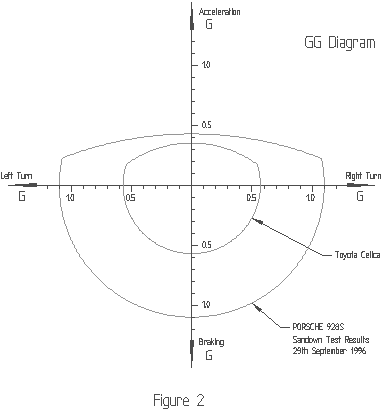
\includegraphics[width=0.96\textwidth]{images/GG_Cars.png}
    \end{columns}
\end{frame}

%TODO Go over trail braking from a G-G curve's perspective

\begin{frame}{How do tires generate force?}
    \onslide<2->{
        \center
        Via friction with the ground
    }
\end{frame}

\begin{frame}{Tires and Friction}
    \begin{block}{Newton's Law of Friction}<+->
        \[F = N\mu\]
        where \(F\) is the max static friction force, \(N\) is the normal force, and \(\mu\) is the static friction coefficient
    \end{block}
    \begin{itemize}
        \onslide<+->{
            \item Tires create force via \textbf{static friction}
                \begin{itemize}
                    \item A tire is in \textit{kinetic} friction if it's locked up or doing a burnout
                \end{itemize}
            }
        \onslide<+->{
            \item \(\mu\) is generally assumed to be constant
                \begin{itemize}
                    \item So \(F\) is linearly dependent on \(N\)
                \end{itemize}
            }
    \end{itemize}
\end{frame}

\begin{frame}{Tires and Load Sensitivity}
    \begin{columns}
        \column{0.65\textwidth}
        \begin{itemize}
            \onslide<+->{
                \item Tires \textbf{do not} have a constant \(\mu\):
                    \[F = N \mu(N)\]
                }
            \item<+-> This phenomena is known as \textbf{Load Sensitivity}
                \onslide<+->{
                \item Generally, \(\mu\) and \(N\) are inversely proportional
                    \begin{itemize}
                        \item As \(\uparrow N\), \(\downarrow \mu\)
                    \end{itemize}
                }
        \end{itemize}

        \column{0.35\textwidth}
        \includegraphics<1->[width=\textwidth]{images/TireLoadSensitivity.jpg}
    \end{columns}
    \begin{alertblock}{\textbf{Load Sensitivity is the singular most impactful thing in racecar design}}<+->
        It alters practically every single decision
    \end{alertblock}
\end{frame}

\begin{frame}{Load Transfer}
    \begin{columns}
        \column{0.5\textwidth}
        \begin{block}{Load Transfer}<+->
            \begin{itemize}
                \item<+-> Weight of vehicle shifting due to acceleration
                \item<+-> Caused by torque of tires against CG, \textit{not by body roll}
            \end{itemize}
        \end{block}

        \begin{itemize}
            \item<+-> \textbf{Reduces global vehicle grip due to load sensitivity}
        \end{itemize}
        \column{0.5\textwidth}
        \includegraphics<3->[width=\textwidth]{images/LoadTransferDiagram.jpg}
    \end{columns}
\end{frame}

\begin{frame}{Load Transfer Example}
    \begin{columns}
        \column{0.6\textwidth}

        \begin{exampleblock}{No load transfer vs 50\% load transfer}<1->
            Assume 4.5kN of static vertical load on each tire.
            \onslide<2->{
                Static traction:
                \[F(4.5\mathrm{kN}) = 5.55\mathrm{kN} \ \Rightarrow \ F^\mathrm{static}_\mathrm{tot} = 5.55 \cdot 4 = 22.2\mathrm{kN}\]
            }
            \onslide<3->{
                With load transfer:
                \begin{equation*}
                    \begin{aligned}
                        F(0.5 \cdot 4.5\mathrm{kN} = 2.25\mathrm{kN}) &= 2.7\mathrm{kN} \\
                        F(1.5 \cdot 4.5\mathrm{kN} = 6.75\mathrm{kN}) &= 7.5\mathrm{kN} \\
                        \onslide<4->{
                        \therefore F^\mathrm{transfer}_\mathrm{tot} = 2(2.7\mathrm{kN} &+ 7.5\mathrm{kN}) = 20.4\mathrm{kN}
                    }
                    \end{aligned}
                \end{equation*}
            }
            \onslide<5->{
                \textbf{8\% Drop in total traction!}
            }
        \end{exampleblock}

        \column{0.4\textwidth}
    \begin{tikzpicture}

    % Include the image in a node
    \node [
        above right,
        inner sep=0] (image) at (0,0) {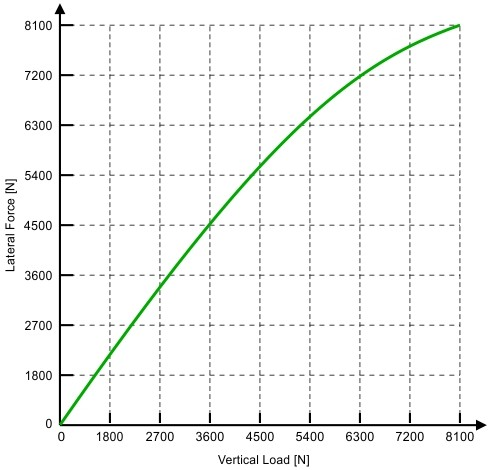
\includegraphics[width=\textwidth]{images/TireLoadSensitivity.jpg}};

    % Create scope with normalized axes
    \begin{scope}[
    x={($0.1*(image.south east)$)},
    y={($0.1*(image.north west)$)}]

    % % Grid
    %     \draw[lightgray,step=1] (image.south west) grid (image.north east);
    %
    % % Axes' labels
    %     \foreach \x in {0,1,...,10} { \node [below] at (\x,0) {\x}; }
    %     \foreach \y in {0,1,...,10} { \node [left] at (0,\y) {\y};}
    %
        % \coordinate (midx) at ($(image) + (5.25,1)$);
        \coordinate (midx) at (5.25,1);
        \coordinate (midc) at (5.25,6.4);
        \coordinate (midy) at (1.2,6.4);

        \coordinate (lowx) at (2.65,1);
        \coordinate (lowc) at (2.65,3.1);
        \coordinate (lowy) at (1.2,3.1);

        \coordinate (highx) at (7.9,1);
        \coordinate (highc) at (7.9,8.76);
        \coordinate (highy) at (1.2,8.76);

        \coordinate (totaly) at (1.2,5.8);

        \draw<2->[line width=1.5pt, blue] (midx)--(midc)--(midy);
        \draw<3->[dashed,line width=1.5pt, red] (lowx)--(lowc)--(lowy);
        \draw<3->[dashed,line width=1.5pt, red] (highx)--(highc)--(highy);
        \draw<4-> (totaly) node[cross=5pt,red, line width=1.5pt]{};

    \end{scope}

    \end{tikzpicture}
    \end{columns}
\end{frame}

%TODO Add "Anatomy of a Corner"
% How does a car turn?
% Answer: It uses the tires to generate a side-force to redirect the car and a torque to rotate the car

\section{Vehicle Balance and Control}
\begin{frame}{How does a car turn?}
    \onslide<+->{}
    \begin{block}{}<+->
        The car uses the tires to generate a \textbf{lateral force to redirect the car} and a \textbf{torque to rotate the car}
    \end{block}
    \onslide<+->{Corners represent a change in two different things:}
    \begin{enumerate}
        \item<+-> Change in \textbf{position}
            \begin{itemize}
                \item<.-> The path the car takes on track
                \item<.-> Governed by \underline{Conservation of (linear) Momentum} (\(F=ma\))
            \end{itemize}
        \item<+-> Change in \textbf{orientation}
            \begin{itemize}
                \item<.-> The direction of the car along the taken path
                \item<.-> Governed by \underline{Conservation of \textit{Angular} Momentum} (\(M=I\alpha\))
            \end{itemize}
    \end{enumerate}

    \begin{itemize}
        \item<+-> Previous topics primarily cover vehicle dynamics for translation
        \item<+-> Now we'll cover orientation/rotation
    \end{itemize}
\end{frame}

\begin{frame}{Angular Momentum}
    \begin{block}{Conservation of Angular Momentum}<+->
        \[M=I\alpha\]
        where \(M\) is the moments (torque) acted on the car, \(I\) is the moment of inertia, and \(\alpha\) is the angular acceleration
    \end{block}
    \begin{itemize}
        \item<+-> Analogous to conservation of linear momentum:
            \onslide<.->{
                \begin{table}[]
                    \begin{tabular}{r|cc}
                                            & Linear & Angular     \\ \hline
                        External Action               & \(F\)  & \(M\)       \\
                        Object's resistance to change & \(m\)  & \(I\)       \\
                        Rate of Change                & \(a\)  & \(\alpha \) \\
                        State Variable                & \(V\)  & \(\omega\) 
                    \end{tabular}
                \end{table}
            }
        \item<+-> Moments can be calculated from a force \(F\) and distance \(r \) via \(M=F\times r\)
    \end{itemize}

\end{frame}

\begin{frame}{Angular Acceleration for Racecars}
    \begin{itemize}
        \item<+-> Reminder: Angular momenum governs \textbf{car orientation}
        \item<+-> Angular velocity \(\omega\) has no direct impact on lap time
        \item<+-> Therefore, we \textit{do not} want to maximize angular acceleration.
        \item<+-> We only want to \textbf{control it such that we can maximize linear acceleration}.
    \end{itemize}
    \begin{alertblock}{This is where balance and control comes into play}<+->
        Ensure that the car is oriented such that we can achieve maximum linear acceleration
    \end{alertblock}
\end{frame}

\begin{frame}{Vehicle Balance}
    \center
    Why do Formula 1 and Indy cars have larger tires at the rear than the front?
\end{frame}

\begin{frame}{Vehicle Balance - Formula 1 Car}
    Balance the moments of the car \hspace{20pt} \(M = \textcolor{orange}{F} \times \textcolor{blue}{r}\)
    \center
    \begin{tikzpicture}

    % Include the image in a node
    \node [
        above right,
        inner sep=0] (image) at (0,0) {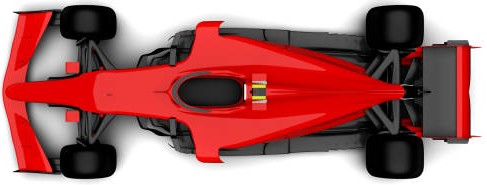
\includegraphics[width=0.8\textwidth]{images/car_overhead.jpg}};

    % Create scope with normalized axes
    \begin{scope}[
    x={($0.1*(image.south east)$)},
    y={($0.1*(image.north west)$)}]

    % % Grid
    %     \draw[lightgray,step=1] (image.south west) grid (image.north east);
    %
    % % Axes' labels
    %     \foreach \x in {0,1,...,10} { \node [below] at (\x,0) {\x}; }
    %     \foreach \y in {0,1,...,10} { \node [left] at (0,\y) {\y};}

        \coordinate (cg) at (6,5);
        \coordinate (fl) at (1.8,1.2);
        \coordinate (fr) at (1.8,8.85);
        \coordinate (rr) at (8.1,8.5);
        \coordinate (rl) at (8.1,1.5);

        \draw (fl) node[cross=8pt,red, line width=1.5pt]{};
        \draw (fr) node[cross=8pt,red, line width=1.5pt]{};
        \draw (rr) node[cross=8pt,red, line width=1.5pt]{};
        \draw (rl) node[cross=8pt,red, line width=1.5pt]{};

        \draw[line width=2.5pt, blue, -stealth] (cg) -- (fl);
        \draw[line width=2.5pt, orange, -stealth] (fl) -- ++(275:1.3);
        \draw[line width=2.5pt, blue, -stealth] (cg) -- (fr);
        \draw[line width=2.5pt, orange, -stealth] (fr) -- ++(275:4.3);
        \draw[line width=2.5pt, blue, -stealth] (cg) -- (rr);
        \draw[line width=2.5pt, orange, -stealth] (rr) -- ++(260:5.3);
        \draw[line width=2.5pt, blue, -stealth] (cg) -- (rl);
        \draw[line width=2.5pt, orange, -stealth] (rl) -- ++(260:1.9);

        \path (cg) pic {cg=8pt};
    \end{scope}

    \end{tikzpicture}
\end{frame}

\begin{frame}{Vehicle Balance - Delta Wing}
    Balance the moments of the car \hspace{20pt} \(M = \textcolor{orange}{F} \times \textcolor{blue}{r}\)
    \center
    \begin{tikzpicture}

    % Include the image in a node
    \node [
        above right,
        inner sep=0] (image) at (0,0) {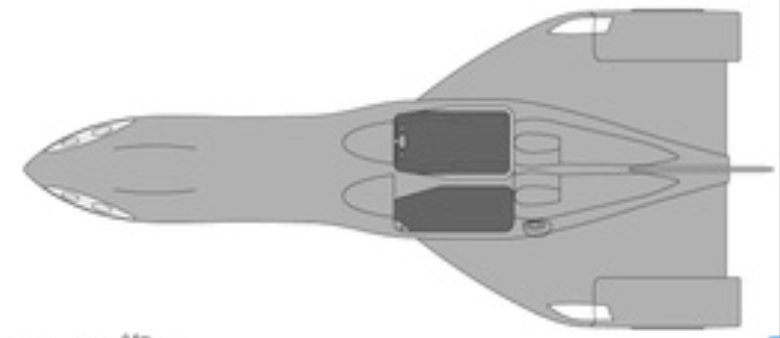
\includegraphics[width=0.8\textwidth]{images/deltawing_overhead.png}};

    % Create scope with normalized axes
    \begin{scope}[
    x={($0.1*(image.south east)$)},
    y={($0.1*(image.north west)$)}]

    % % Grid
    %     \draw[lightgray,step=1] (image.south west) grid (image.north east);
    %
    % % Axes' labels
    %     \foreach \x in {0,1,...,10} { \node [below] at (\x,0) {\x}; }
    %     \foreach \y in {0,1,...,10} { \node [left] at (0,\y) {\y};}

        \coordinate (cg) at (7.5,5);
        \coordinate (fl) at (2.05,3.8);
        \coordinate (fr) at (2.05,6.05);
        \coordinate (rr) at (8.5,9);
        \coordinate (rl) at (8.5,1);

        \draw (fl) node[cross=8pt,red, line width=1.5pt]{};
        \draw (fr) node[cross=8pt,red, line width=1.5pt]{};
        \draw (rr) node[cross=8pt,red, line width=1.5pt]{};
        \draw (rl) node[cross=8pt,red, line width=1.5pt]{};

        \draw[line width=2.5pt, blue, -stealth] (cg) -- (fl);
        \draw[line width=2.5pt, orange, -stealth] (fl) -- ++(275:1.0);
        \draw[line width=2.5pt, blue, -stealth] (cg) -- (fr);
        \draw[line width=2.5pt, orange, -stealth] (fr) -- ++(275:1.5);
        \draw[line width=2.5pt, blue, -stealth] (cg) -- (rr);
        \draw[line width=2.5pt, orange, -stealth] (rr) -- ++(260:4.3);
        \draw[line width=2.5pt, blue, -stealth] (cg) -- (rl);
        \draw[line width=2.5pt, orange, -stealth] (rl) -- ++(260:1.9);

        \path (cg) pic {cg=8pt};
    \end{scope}

    \end{tikzpicture}
\end{frame}

\begin{frame}{Oversteer vs Understeer}
    \begin{block}{Neutral Steer}<+->
        Moments in perfect \textit{imbalance}
    \end{block}
    \begin{block}{Under Steer}<+->
        Unbalanced moments cause under-rotation
    \end{block}
    \begin{block}{Over Steer}<+->
        Unbalanced moments cause over-rotation
    \end{block}

    \begin{itemize}
        \item<+-> The latter two prevent achieving maximum linear acceleration 
        \item<+-> A car can dynamically change between all three states
        \item<+-> Changes occur due to differences in load transfer, suspension magic, and through dynamic movement
    \end{itemize}
\end{frame}

\section{Three Tenants of Racecar Design}
\begin{frame}{Three Tenants of Racecar Design}
    \textit{In order of importance:}
    \begin{enumerate}
        \item<+-> Make it Lighter
            \begin{itemize}
                \item<.-> Improves acceleration, load transfer, responsiveness, etc.
            \end{itemize}
        \item<+-> Make it Lower
            \begin{itemize}
                \item<.-> Lowering a component lowers CG \(\Rightarrow\) reduces load transfer
            \end{itemize}
        \item<+-> Make it more Central
            \begin{itemize}
                \item<.-> Reduces \(I\) \(\Rightarrow\) makes the car more responsive
            \end{itemize}
    \end{enumerate}
    \begin{alertblock}{\textbf{The car that is lighter, has a lower CG, or has a lower inertia will be faster}}<+->
    \end{alertblock}

\end{frame}

\begin{frame}{Recommended Resources}

    \begin{itemize}
        \item \textit{Tune to Win} by Carroll Smith
            \begin{itemize}
                \item Vehicle dynamics for normal people
                \item Covers the gamut of racecar design topics (aero, cooling, VD, powertrain, etc.)
            \end{itemize}
        \item \textit{Racecar Vehicle Dynamics} by Milliken \& Milliken
            \begin{itemize}
                \item "The Bible"
                \item It's a textbook, but incredibly useful
                \item More specialized to vehicle dynamics (shocking given the name)
            \end{itemize}
    \end{itemize}
\end{frame}

\begin{frame}{Questions}
\end{frame}

\end{document}
